\documentclass{beamer}
\usepackage{tikz}
\usetikzlibrary{calc}
\usetikzlibrary{arrows.meta}
\usetikzlibrary{backgrounds,matrix,fadings,calc,positioning,decorations.pathreplacing,decorations.markings,arrows.meta,shapes,shapes.multipart}
\usetikzlibrary{patterns,math,quotes,positioning,angles}
\usetikzlibrary{spy}
\usepackage{xcolor}
\usepackage{siunitx}
\usepackage{chemfig}
\usepackage{amsmath}
\usepackage[version=4]{mhchem}
\usepackage[utf8]{inputenc}
\usetheme{Berlin}
\usecolortheme{default}

\title[Condensation and Evaporation of Hexane in Nanoporous Alumina Membranes]{Condensation and Evaporation of Hexane in Nanoporous Alumina Membranes}
%\subtitle{}
\author[Hermann Böttcher]{Hermann Böttcher\inst{1} \and Victor Doebele\inst{2} \and Pierre-Etienne Wolf\inst{2} \and Panayotis Sphatis\inst{2} \and Fabien Souris\inst{2}}
\institute{
          \inst{1}University of Constance
          \and
          \inst{2}Institut Néel, Centre national de la recherche scientifique
          }
\date[Constance, 02/10/2018]{02/10/2018}
%\logo{
\includegraphics[height=1.5cm]{graphics/logoNEEL.png}}

\begin{document}

  \frame{\maketitle}

  \begin{frame}{Overview}
      \begin{enumerate}
        \item Context
        \item Goals of the internship
        \item Theoretical background
        \item Experimental setup
        \item Conclusions
      \end{enumerate}
  \end{frame}

  \begin{frame}{Context}
    \begin{block}{Grand scheme}
      \begin{itemize}
        \item Condensation and evaporation of fluids in confinement
        \pause

        \item Dependency on
          \begin{itemize}
            \item pore diameter
            \item temperature (relative to the critical temperature)
          \end{itemize}
      \end{itemize}
    \end{block}
    \pause

    \begin{block}{Plan}
      \begin{itemize}
        \item Anodized alumina membranes (AAM)
        \item Test setup using Hexane $\rightarrow$ working at room temperature permits much faster executable experiments
        \item Transfer to \textbf{helium} experiment
      \end{itemize}
    \end{block}
  \end{frame}

  \begin{frame}{Goals}
    \begin{itemize}
      \pause
      \item Improving and \textbf{systemizing} the evaluation of the recorded isotherm data

      \item Performing isotherm measurements on many membranes for \textbf{statistics}
      \pause

      \item Comparing the pore diameters extracted from the volumetric measurements those from scanning electron microscopy (SEM) images
      \pause

      \item Improving the fabrication process to reduce the dispersion
      \pause

      \item Testing the efficiency of the ALD process as a means to reduce the pore diameters
    \end{itemize}
  \end{frame}

  \begin{frame}{Membrane production}
         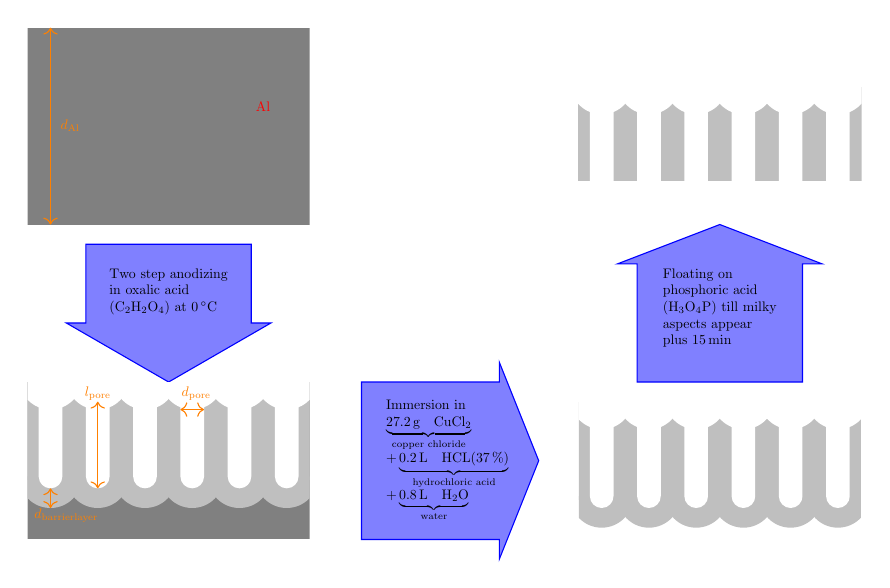
\begin{tikzpicture}[scale=0.5, transform shape,
                             MyArrow/.style={single arrow, draw, minimum width=16mm, minimum height=12mm,
                             inner sep=0mm, single arrow head extend=2mm}]
             %\tikzset{fontscale/.style = {font=\relsize{#1}}}
             \tikzset{MyArrow/.style={single arrow, draw, minimum width=16mm, minimum height=10mm, inner sep=0mm, single arrow head extend=.8mm}}
           \begin{scope}
              \def\l{7.2};
              \def\h{5};
              \def\d{0.8};
              %\node[draw = blue!70, fill = blue!50, MyArrow, rotate=270] at (2.6, -2) {\phantom{arrow}};
              %\node[anchor=west, align=left] at (3.6,-2) {Two step anodizing\\ in oxalic acid\\ (\ce{C2H2O4}) at $\SI{0}{\celsius}$};
              %\draw[fill=blue!50, color=blue] (3.6,-3)--(2.6,-2)--(3.1,-2)--(3.1,-1)--(4.2,-1)--(4.2,-2)--(4.6,-2)--(3.6,-3);
              \fill[color=blue!50, draw=blue] (1.5,-.5)--(5.7,-.5)--(5.7,-2.5)--(6.2,-2.5)--(3.6,-4)--(1,-2.5)--(1.5,-2.5)--cycle;
              \node[anchor=north, align=left] at (3.6,-1) {Two step anodizing\\ in oxalic acid\\ (\ce{C2H2O4}) at $\SI{0}{\celsius}$};
              \clip (0.02,0) rectangle (\l - 0.02,\h);
              \fill[gray] (0,0) rectangle (\l,\h);
              \draw[color=orange,<->] (0.6,0) -- (0.6,\h);
              \node[color=orange] at (1.1,\h/2) {$d_\mathrm{Al}$};
              \node[color=red] at (6,3) {$\ce{Al}$};
           \end{scope}
           \begin{scope}[yshift=-8cm]
               \def\l{7.2};
               \def\h{4};
               \def\d{0.6};
               %\node[draw = blue!70, fill = blue!50, MyArrow] at (11, 2) {\phantom{arrow}};
               %\node[anchor=south, align=left] at (11,3) {Immersion in\\ $\underbrace{\SI{27,2}{\gram}\quad\ce{CuCl2}}_{\text{copper chloride}}$\\ $ + \underbrace{\SI{0,2}{\l}\quad\ce{HCL}(\SI{37}{\percent})}_{\text{hydrochloric acid}}$\\ $+ \underbrace{\SI{0,8}{\l}\quad\ce{H2O}}_{\text{water}}$};
               \fill[color=blue!50, draw=blue] (8.5,0)--(8.5,4)--(12,4)--(12,4.5)--(13,2)--(12,-.5)--(12,0)--cycle;
               \node[anchor=west, align=left] at (9,2) {Immersion in\\ $\underbrace{\SI{27,2}{\gram}\quad\ce{CuCl2}}_{\text{copper chloride}}$\\ $ + \underbrace{\SI{0,2}{\l}\quad\ce{HCL}(\SI{37}{\percent})}_{\text{hydrochloric acid}}$\\ $+ \underbrace{\SI{0,8}{\l}\quad\ce{H2O}}_{\text{water}}$};
               \begin{scope}
               \clip (0.02,0) rectangle (\l - 0.02,\h);
               \fill[gray] (0,0) rectangle (\l,\h);
               \fill[lightgray] (0,1.5) rectangle (\l,\h);
               \foreach \i in {1,3,...,11}{
                   \fill[white] (- 4 / 3 * \d + \i * \d, \h + 0.1) arc (180:360:\d / 3 * 4);
                   \fill[lightgray] (- 4 / 3 * \d + \i * \d, \h - 2.5 + 0.1) arc (180:360:\d / 3 * 4);
                   \fill[white] (-0.5 * \d + \i * \d, \h - 2.5 + 0.1) arc (180:360:\d / 2) -- (-0.5 * \d + \i * \d + \d, \h + 0.1) -- (-0.5 * \d + \i * \d, \h + 0.1) -- cycle;}
               \draw[color=orange,<->] (3.9,3.3) -- (4.5,3.3);
               \node[color=orange] at (4.3,3.7) {$d_\mathrm{pore}$};
               \draw[color=orange,<->] (0.6,\h-2.5+0.1-0.3) -- (0.6,\h-2.5+0.1-0.8);
               \node[color=orange] at (1,\h-2.5+0.1-0.8-0.2) {$d_\mathrm{barrier layer}$};
               \draw[color=orange,<->] (1.8,\h-2.5+0.1-0.3) -- (1.8,\h-+0.1-0.4);
               \node[color=orange] at (1.8,\h-0.3) {$l_\mathrm{pore}$};
               \end{scope}
            \end{scope}
            \begin{scope}[yshift=-8cm, xshift=14cm]
                \def\l{7.2};
                \def\h{3.5};
                \def\d{0.6};
                %\node[draw = blue!70, fill = blue!50, MyArrow, rotate=90] at (4.6, 6) {\phantom{arrow}};
                %\node[anchor=east, align=left] at (4.6,6) {Floating on\\ phosphoric acid\\ (\ce{H3O4P})};
                \fill[color=blue!50, draw=blue] (1.5,4)--(5.7,4)--(5.7,7)--(6.2,7)--(3.6,8)--(1,7)--(1.5,7)--cycle;
                \node[anchor=north, align=left] at (3.6,7) {Floating on\\ phosphoric acid\\ (\ce{H3O4P}) till milky\\ aspects appear\\ plus $\SI{15}{\minute}$};
                \begin{scope}
                \clip (0.02,0) rectangle (\l - 0.02,\h);
                %\fill[gray] (0,0) rectangle (\l,\h);
                \fill[lightgray] (0,1) rectangle (\l,\h);
                \foreach \i in {1,3,...,11}{
                    \fill[white] (- 4 / 3 * \d + \i * \d, \h + 0.1) arc (180:360:\d / 3 * 4);
                    \fill[lightgray] (- 4 / 3 * \d + \i * \d, \h - 2.5 + 0.1) arc (180:360:\d / 3 * 4);
                    \fill[white] (-0.5 * \d + \i * \d, \h - 2.5 + 0.1) arc (180:360:\d / 2) -- (-0.5 * \d + \i * \d + \d, \h + 0.1) -- (-0.5 * \d + \i * \d, \h + 0.1) -- cycle;}
                \end{scope}
            \end{scope}
            \begin{scope}[xshift=14cm]
                \def\l{7.2};
                \def\h{3.5};
                \def\d{0.6};
                \begin{scope}
                \clip (0,0) rectangle (\l,\h);
                \fill[lightgray] (0,1.1) rectangle (\l,\h);
                \foreach \i in {1,3,...,11}{
                    \fill[white] (- 4 / 3 * \d + \i * \d, \h + 0.1) arc (180:360:\d / 3 * 4);
                    \fill[white] (-0.5 * \d + \i * \d, \h - 2.5 + 0.1) arc (180:360:\d / 2) -- (-0.5 * \d + \i * \d + \d, \h + 0.1) -- (-0.5 * \d + \i * \d, \h + 0.1) -- cycle;}
                \end{scope}
            \end{scope}
         \end{tikzpicture}
  \end{frame}

  \begin{frame}{Alumina membranes}
    \begin{columns}[onlytextwidth, T]
      \column{\dimexpr\linewidth / 2}
        %\vspace{-2.5cm}

        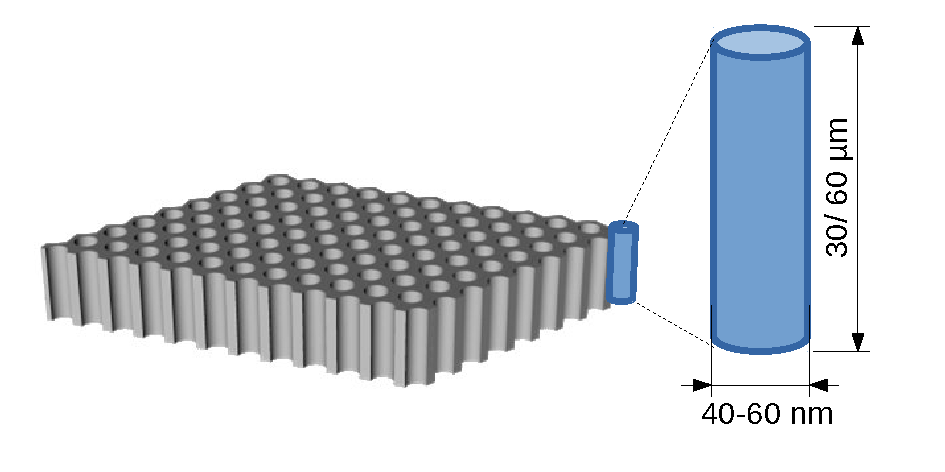
\includegraphics[width=\linewidth]{images/membranes.pdf}

        \column{\dimexpr\linewidth / 2}

        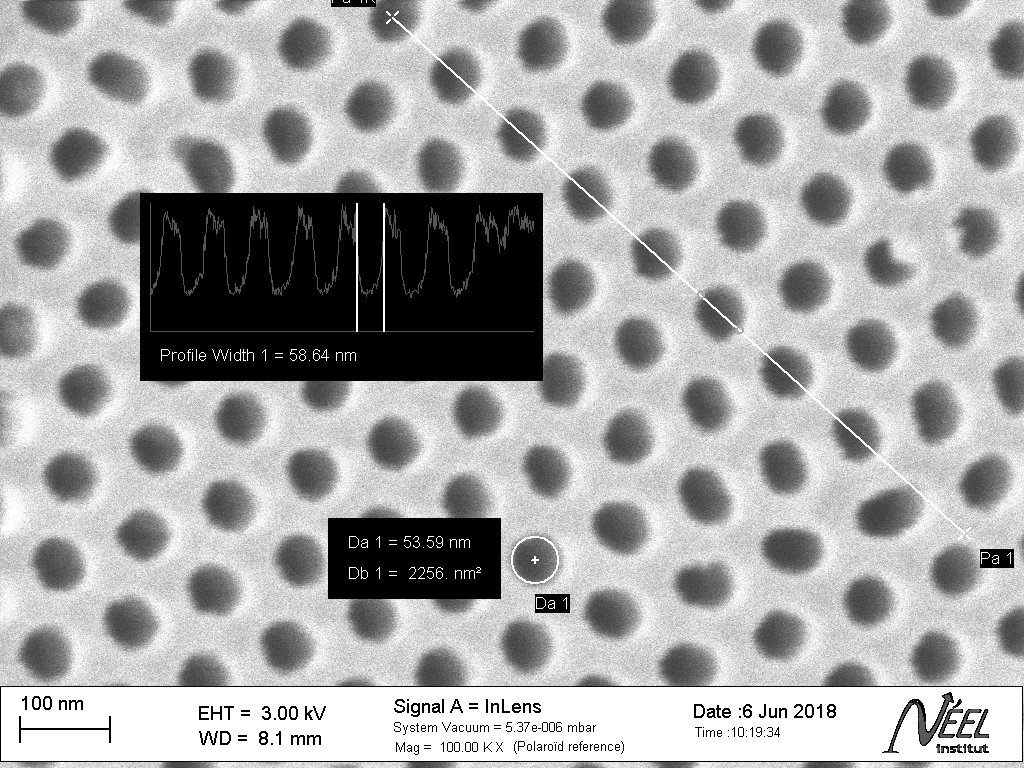
\includegraphics[width=0.7\linewidth]{images/295c__al_side.jpg}
        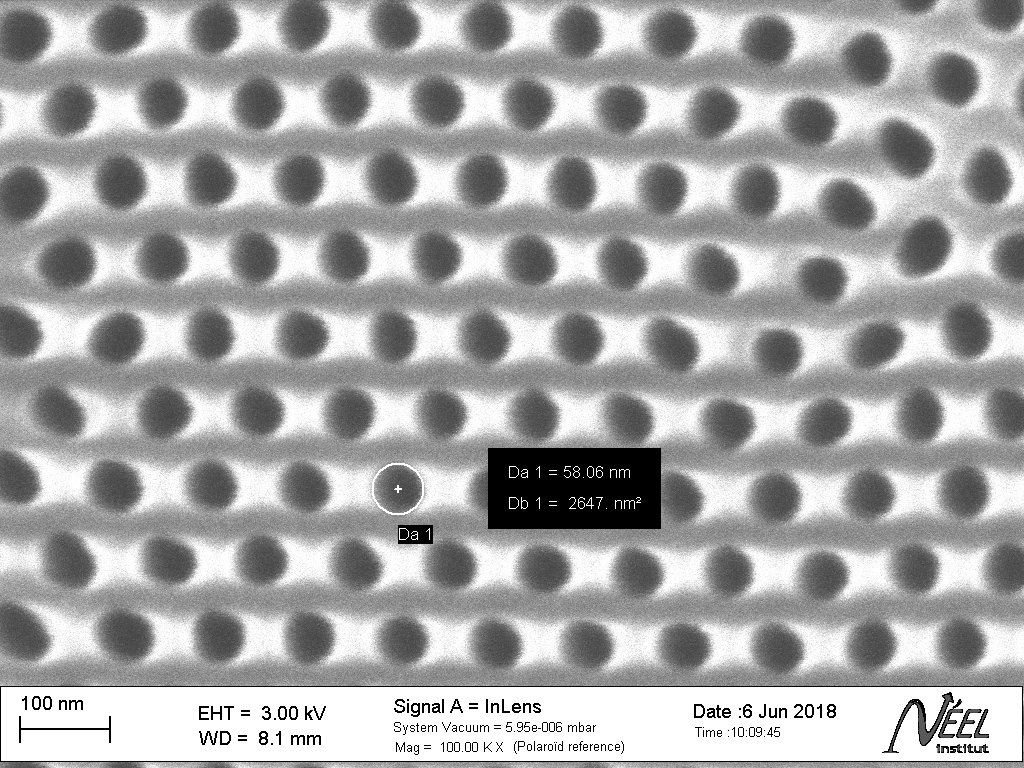
\includegraphics[width=0.7\linewidth]{images/295c_sol_side.jpg}
    \end{columns}
  \end{frame}

  \begin{frame}{Experimental setup}

  \end{frame}

  \begin{frame}{Data evaluation}

  \end{frame}

  \begin{frame}{Inverse funnelling}

  \end{frame}

  \begin{frame}{Atomic layer deposition}

  \end{frame}


\end{document}
